\section{Research Question}\label{sec:research_question}

As already mentioned above the usage of application specific approaches in networking allows for a reduction in latency.
In this thesis we will consider a media streaming scenario that runs on top of QUIC by using the ``Media over QUIC'' (MoQ) transport protocol
~\parencite{draft-moqtransport}.
The central question we will try to answer in this thesis will then be:
\vspace{0.5cm}
\begin{center}
    \textit{How can we improve the performance of a relay in a media streaming scenario by using eBPF technology?}
\end{center}
\vspace{0.5cm}
with more specific sub-questions being:
\vspace{0.5cm}
\begin{enumerate}
    \item \textit{How can we avoid the need to direct a packet through userspace?}
    \item \textit{How to handle the fact that packets are heavily encrypted?}
    \item \textit{What communication between userspace and eBPF program is necessary to stay coherent with potential state?}
    \item \textit{How can our approach be generalized to other protocols?}
\end{enumerate}
\vspace{0.5cm}
By using eBPF technology together with kernel hook points provided by the Linux-Kernel, we will try to find a setup that improves relay 
performance using eBPF programs that handle basic relay capabilities, such as packet forwarding and congestion control.
Since the QUIC protocol is designed to handle a large portion of its workload in userspace we look into possibilities of delaying any 
userspace processing until \textbf{after} the packet has been forwarded to the client.
This way the raw delay that the packet experiences from the initial media server to the client could be reduced. 
However, since QUIC is a connection oriented protocol, we need to make sure that the QUIC connection state stays 
coherent despite the additional processing steps done by the eBPF program.
We will investigate which additional processing steps are needed in our case, how they compare to challenges when expanding our approach to other
protocols and how they can be implemented in an eBPF program.

\vspace{0.5cm}
\begin{figure}[htbp] % TODO: where to put this?
    \centering
    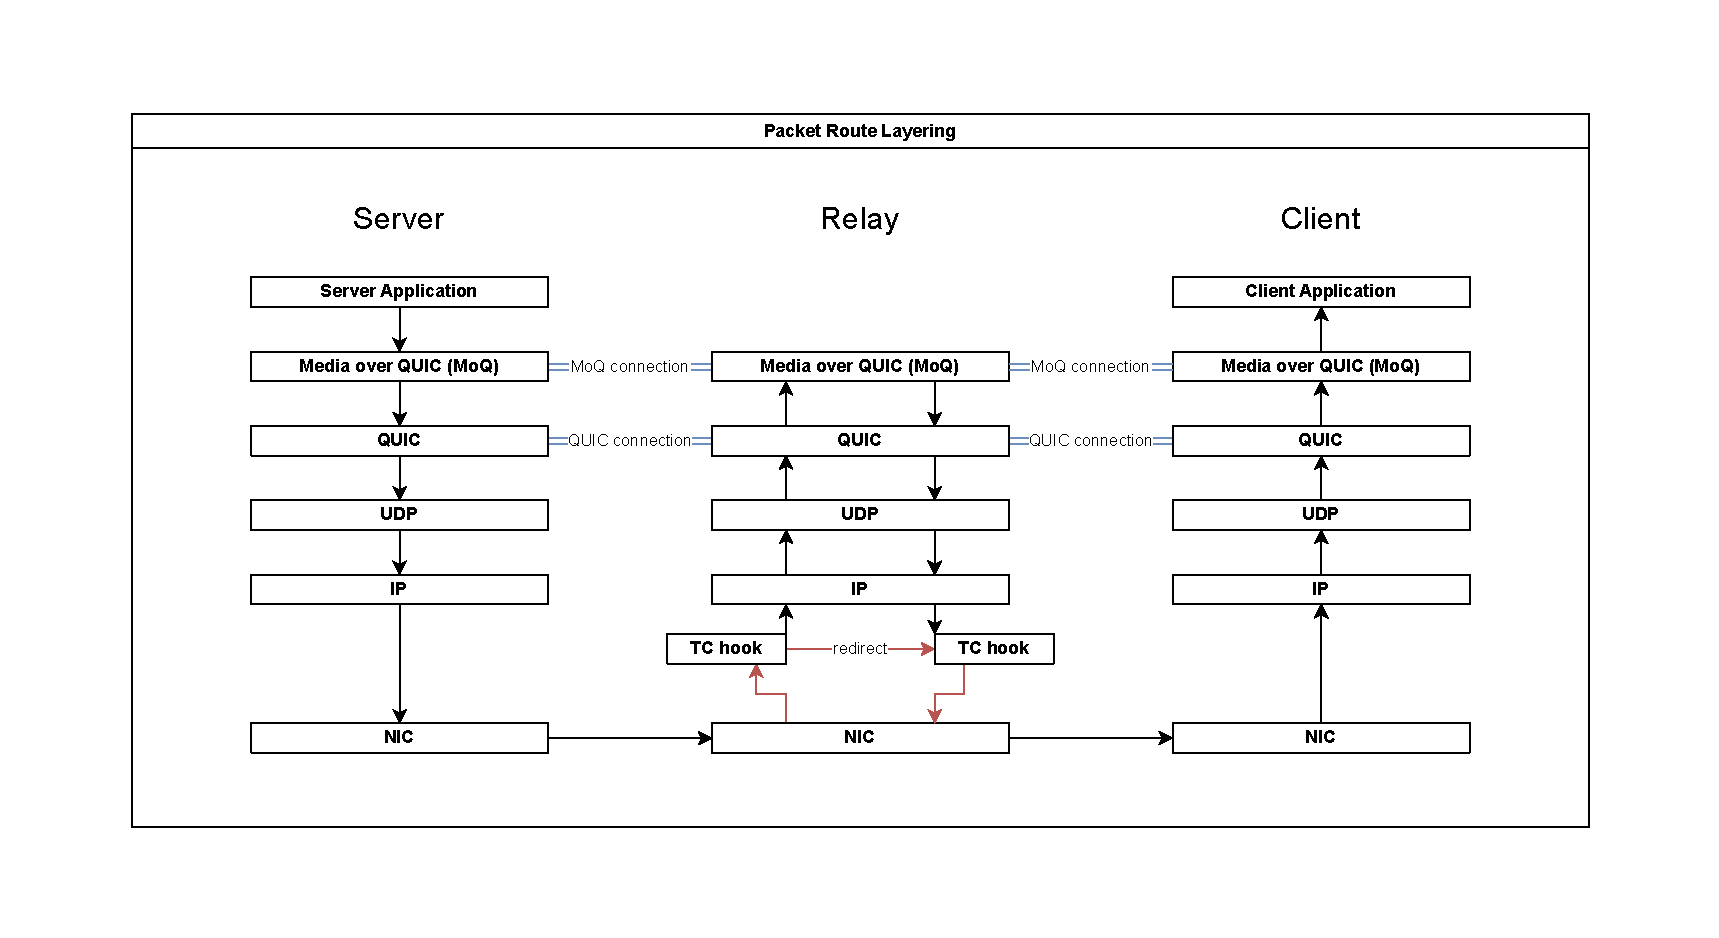
\includegraphics[width=0.7\textwidth]{figures/02_background/route-layering.drawio.pdf}
    \caption[Packet path schematic regarding network stack]{Conventional networking layers a packet passes.
    The red loop indicates again the ``short-cut'' that is utilized by the fast-relay 
    (eBPF packet-forwarding {-} no need to go up to userspace).}\label{fig:route-layering}
\end{figure}